\documentclass[11pt]{article}
\usepackage[margin=1in]{geometry}
\usepackage{amsmath, amssymb, amsthm}
\usepackage{graphicx}
\usepackage{float}
\usepackage{hyperref}
\usepackage{caption}
\usepackage{subcaption}
\usepackage{pgfplots}
\pgfplotsset{compat=1.16}

\title{Advanced Training Metrics and Mathematical Formulations}
\author{Reno-Vans Ensemble System}
\date{\today}

\begin{document}
\maketitle

\section{Introduction}
This document presents the core mathematical formulations and metrics used in our ensemble training pipeline. Key topics include:
\begin{itemize}
    \item Token-level and sequence-level entropy
    \item Logistic regression ensemble for quality scoring
    \item FAISS-based KNN retrieval for similar example search
    \item Cross-model alignment loss for latent space fusion
    \item Knowledge distillation loss for training a student model
\end{itemize}

\section{Entropy Calculations}
For a probability distribution $\mathbf{p} = (p_1, p_2, \dots, p_n)$, the token-level entropy is defined as:
\begin{equation}
    H(\mathbf{p}) = -\sum_{i=1}^{n} p_i \log p_i.
\end{equation}
The sequence-level (mean) entropy over $n$ tokens is given by:
\begin{equation}
    H_{\text{seq}} = \frac{1}{n}\sum_{i=1}^{n} H(p_i).
\end{equation}

\section{Logistic Regression Ensemble}
Our logistic regression ensemble combines features from multiple models. Given a feature vector $\mathbf{x} \in \mathbb{R}^7$, the prediction is:
\begin{equation}
    \hat{y} = \sigma(\mathbf{w}^T \mathbf{x} + b),
\end{equation}
where $\sigma(z) = \frac{1}{1+e^{-z}}$ is the sigmoid function. The features include:
\begin{enumerate}
    \item Primary confidence: $1 - H_{\text{seq}}$ from the primary model.
    \item Secondary confidence: Derived from ensemble disagreement.
    \item Evaluator confidence: $1 - H_{\text{seq}}$ from the evaluator model.
    \item Raw primary sequence entropy.
    \item Ensemble disagreement score.
    \item KNN similarity score.
    \item Example quality metadata.
\end{enumerate}

\section{KNN Retrieval with FAISS}
We use FAISS to build an index for rapid retrieval of similar code examples. For two normalized embeddings $\mathbf{u}$ and $\mathbf{v}$, the cosine similarity is:
\begin{equation}
    \text{similarity}(\mathbf{u}, \mathbf{v}) = \frac{\mathbf{u} \cdot \mathbf{v}}{\|\mathbf{u}\| \|\mathbf{v}\|}.
\end{equation}
A higher similarity indicates a closer match between the query and stored examples.

\section{Cross-Model Alignment Loss}
To ensure consistent latent representations across models, we project their final hidden states into a common space and compute cosine similarities. The alignment loss is defined as:
\begin{equation}
    \mathcal{L}_{\text{align}} = \frac{1}{3} \left[ (1 - \cos(\mathbf{z}_1, \mathbf{z}_2)) + (1 - \cos(\mathbf{z}_1, \mathbf{z}_3)) + (1 - \cos(\mathbf{z}_2, \mathbf{z}_3)) \right],
\end{equation}
where $\mathbf{z}_1$, $\mathbf{z}_2$, and $\mathbf{z}_3$ are the projected representations from the primary, secondary, and evaluator models respectively.

\section{Knowledge Distillation}
In our advanced knowledge distillation, a student MLP is trained to mimic the ensemble projection. The distillation loss is given by:
\begin{equation}
    \mathcal{L}_{\text{distill}} = \left\| f_{\text{student}}(\mathbf{h}) - f_{\text{target}}(\mathbf{h}) \right\|^2,
\end{equation}
where $\mathbf{h}$ represents the hidden state from the primary model, and $f_{\text{student}}$ and $f_{\text{target}}$ are the student and target projection functions, respectively.

\section{Visualization of Training Metrics}
Below is an example plot of simulated training loss and sequence entropy over epochs.

\begin{figure}[H]
    \centering
    \begin{subfigure}[b]{0.45\textwidth}
        \centering
        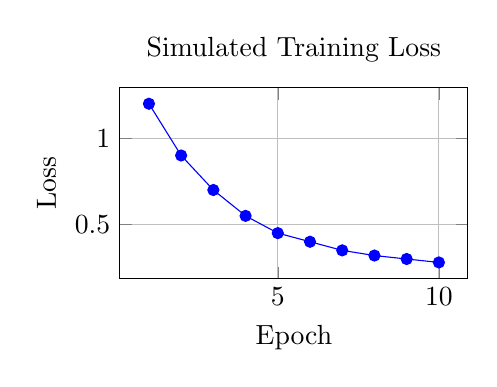
\begin{tikzpicture}
            \begin{axis}[
                xlabel={Epoch},
                ylabel={Loss},
                title={Simulated Training Loss},
                width=6cm,
                height=4cm,
                grid=both
            ]
            \addplot[color=blue, mark=*] coordinates {
                (1,1.20) (2,0.90) (3,0.70) (4,0.55) (5,0.45) (6,0.40) (7,0.35) (8,0.32) (9,0.30) (10,0.28)
            };
            \end{axis}
        \end{tikzpicture}
        \caption{Training Loss}
    \end{subfigure}
    \begin{subfigure}[b]{0.45\textwidth}
        \centering
        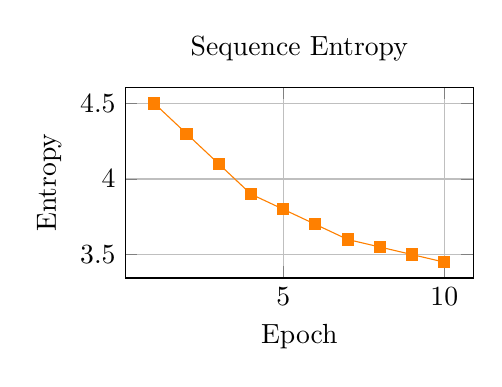
\begin{tikzpicture}
            \begin{axis}[
                xlabel={Epoch},
                ylabel={Entropy},
                title={Sequence Entropy},
                width=6cm,
                height=4cm,
                grid=both
            ]
            \addplot[color=orange, mark=square*] coordinates {
                (1,4.50) (2,4.30) (3,4.10) (4,3.90) (5,3.80) (6,3.70) (7,3.60) (8,3.55) (9,3.50) (10,3.45)
            };
            \end{axis}
        \end{tikzpicture}
        \caption{Sequence Entropy}
    \end{subfigure}
    \caption{Simulated Training Metrics over 10 Epochs}
\end{figure}

\section{Conclusion}
This document has provided a detailed mathematical formulation of the key components of our ensemble training pipeline. By leveraging these formulations, we can monitor, analyze, and improve the system's performance continuously.

\end{document}
